%
% kugelschnitt.tex
%
\begin{figure}
\centering
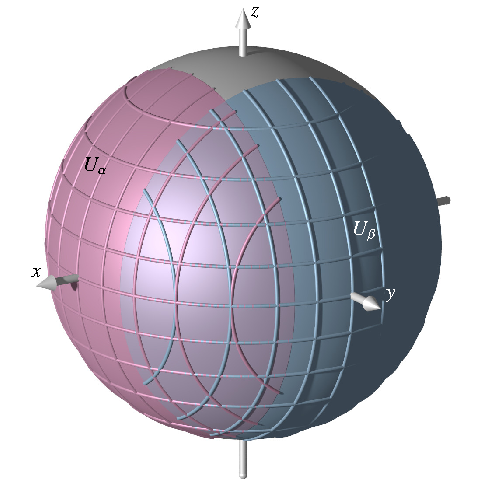
\includegraphics{chapters/030-gruppen/images/kugelschnitt.pdf}
\caption{Zwei Karten der Kugeloberfläche und deren Schnittbereich.
Differenzierbarkeit von Funktionen auf der Kugeloberfläche kann mit
Hilfe der Karten nur dann definiert werden, wenn die Kartenwechselabbildung
$\varphi_\alpha\circ\varphi_\beta^{-1}$ und
$\varphi_\beta\circ\varphi_\alpha^{-1}$ differenzierbare Abbildungen
zwischen offenen Mengen in $\mathbb{R}^n$ sind.
\label{buch:gruppen:gruppe:fig:kugelkartenwechsel}}
\end{figure}
